\section{Wykład I}
\subsection{Tematyka wykładu.}

Idea, która nam przyświeca,to poszerzenie wiedzy, którą nabyło się na podstawowym wykładzie z Logiki dla Informatyków. Chcemy popatrzeć na kilka kwestii związanych z logiką m.in. systemy wnioskowania oraz semantyka tych systemów. Zaczniemy od Algebry Uniwersalnej. Poniżej plan przedmiotu.

\subsection{Podstawowe definicje.}

\begin{definition}{Zbiór częściowo uporządkowany}

	Niech $X$ będzie zbiorem. Na jego produkcie, czyli zbiorze $X \times X$ określamy relację $\le\text{ }\subseteq X\times X$, spełniającą następujące warunki:
	\begin{itemize}
		\item Zwrotność:
			\[
			\left( \forall x\in X \right) x \le x 
			.\] 
		\item Przechodniość:
			\[
			\left( \forall x,y,z \in X \right) x\le y \land y \le  z \implies x \le z  
			.\] 
		\item Słaba antysymetryczność:
			\[
			\left( \forall x,y\in X \right) x\le y \land y\le x \implies x = y 
			.\] 
	\end{itemize}
\end{definition}

W dalszej części wykładu będziemy używać angielskiej nazwy zbioru częściowo uporządkowanego, mianowicie \textbf{poset}(partially ordered set).

\begin{definition}{Elementy największy i najmniejszy posetu}
	

\end{definition}

\begin{definition}{Element maksymalny i minimalny posetu}
	

\end{definition}

\begin{definition}{Ograniczenie górne i ograniczenie dolne oraz kres górny i kres dolny posetu}
	
	Niech $\left( P, \le  \right) $ posetem oraz $X\subseteq P$. Element $a \in P$ jest \textbf{ograniczeniem górnym}  zbioru $X$ jeśli dla każdego $x \in  X$ zachodzi $x \le a$. 

	\textbf{Kresem górnym} zbioru $X$ nazywamy najmniejszy element zbioru $\{a : a \text{ograniczeniem górnym zbioru X}\} $
\end{definition}

Przykłady posetów:
\begin{itemize}
	\item $(\N, \le )$- zbiór liczb naturalnych z relacją 'słabej' nierówności
	\item $(\N, |)$- zbiór liczb naturalnych z relacją podzielności.
	\item $(A, \subseteq )$- dowolny zbiór A z relacją zawierania się.
\end{itemize}
\subsection{Diagramy Hassego}

Do pokazywania posetów wygodnie jest używać diagramów Hassego.

Przykładowe diagramy Hassego:

\begin{figure}[H]
    \begin{minipage}{0.3\textwidth}
        \centering
\begin{tikzpicture}[node distance=1cm]
    % Wiersz 1
    \node (abc) at (0,0) {$\{a,b,c\}$};

    % Wiersz 2
    \node [below=of abc, xshift=-1.2cm] (ab) {$\{a,b\}$};
    \node [below=of abc] (bc) {$\{b,c\}$};
    \node [below=of abc, xshift=1.2cm] (ac) {$\{a,c\}$};

    % Wiersz 3
    \node [below=of ab] (a) {$\{a\}$};
    \node [below=of bc] (b) {$\{b\}$};
    \node [below=of ac] (c) {$\{c\}$};
    
    % Wiersz 4
    \node [below=of b] (O) {$\emptyset$};

    % Rysowanie krawędzi
    \draw (abc) -- (ab);
    \draw (abc) -- (bc);
    \draw (abc) -- (ac);

    \draw (ab) -- (a);
    \draw (ab) -- (b);

    \draw (bc) -- (b);
    \draw (bc) -- (c);
    
    \draw (ac) -- (a);
    \draw (ac) -- (c);
    
    \draw (a) -- (O);
    \draw (b) -- (O);
    \draw (c) -- (O);
\end{tikzpicture}
       \caption{Zbiór $\{a,b,c\}$ z relacją inkluzji $\subseteq$}
    \end{minipage}
    \hfill
    \begin{minipage}{0.15\textwidth}
        \centering
	\begin{tikzpicture}[node distance=0.6cm]
		\node  (inf) at (0,0) {$\vdots$};
		\node [below=of inf] (3) {$3$};
		\node [below=of 3] (2) {$2$};
		\node [below=of 2] (1) {$1$};
		\node [below=of 1] (0) {$0$};
		
		\draw (0) -- (1) -- (2) -- (3) -- (inf);	
		
        \end{tikzpicture}
        \caption{Zbiór $\N$ z relacją 'mniejszy lub równy' $\le $} 
    \end{minipage}
    \hfill
 \begin{minipage}{0.45\textwidth}
        \centering
	\begin{tikzpicture}[node distance= 0.6cm]
		% Pierwszy wiersz
		\node (0) at (0,0) {$0$};
		% Drugi wiersz
		\node [below=of 0, xshift=-2.15cm] (8) {$8$};
		\node [below=of 0] (20) {$20$};
		\node [left=of 20] (12) {$12$};
		\node [right=of 20] (30) {$30$};
		\node [below=of 0, xshift=2.15cm, yshift=-0.2cm] (2inf) {$\dots$};
		% Trzeci wiersz
		\node [below=of 8] (4) {$4$};
		\node [below=of 12] (6) {$6$};
		\node [below=of 20] (10) {$10$};
		\node [below=of 30] (15) {$15$};
		\node [below=of 2inf, yshift=-0.18cm] (3inf) {$\ldots$};	
		% Czwarty wiersz
		\node [below=of 4] (2) {$2$};
		\node [below=of 6] (3) {$3$};
		\node [below=of 10] (5) {$5$};
		\node [below=of 15] (7) {$7$};
		\node [below=of 3inf, yshift=-0.2cm] (4inf) {$\ldots$};
		% Piąty wiersz
		\node [below=of 5] (1) {$1$};

		\draw (1) -- (2) -- (4) -- (8);
		\draw (1) -- (3) -- (6) -- (12);
		\draw (1) -- (5) -- (10) -- (20);
		\draw (1) -- (7) -- (15) -- (30);
		\draw (2) -- (6) --  (30);
		\draw (2) -- (10) -- (30);
		\draw (3) -- (15);
		\draw (5) -- (15);
		\draw [dotted] (1) -- (4inf);
		
		\draw (4) -- (12);
		\draw (4) -- (20);
		\draw [dotted] (2) -- (3inf);
		\draw [dotted] (3) -- (3inf);
		\draw [dotted] (5) -- (3inf);
		\draw [dotted] (7) -- (3inf);
		\draw [dotted] (4inf) -- (3inf);
		
		\draw [dotted] (4) -- (2inf);
		\draw [dotted] (6) -- (2inf);
		\draw [dotted] (10) -- (2inf);
		\draw [dotted] (15) -- (2inf);
		\draw [dotted] (3inf) -- (2inf);
		
		\draw [dotted] (30)   -- (0);
		\draw [dotted] (2inf) -- (0);		
		\draw [dotted] (20)   -- (0);
		\draw [dotted] (12)   -- (0);
		\draw [dotted] (8)   -- (0);
        \end{tikzpicture}
        \caption{Zbiór liczb $\N$ z relacją podzielności $|$}
    \end{minipage}
\end{figure}

\begin{definition}{Dualność}
	
	Niech $(P,\le )$ będzie posetem. Porządek $(P, \le^{-1})$ nazywamy porządkiem \textbf{dualnym} do $(P,\le)$.
	Jeżeli dane jest pojęcie $Q$ dotyczące porządków, to pojęcie $Q^{-1}$ dualne do niego, otrzymujemy poprzez zastąpienie w definicji $Q$ 
	symbolu $\le $ przez symbol $\le^{-1}$. Zauważmy, że pojęcia maksymalny i minimalny oraz największy i najmniejszy są do siebie dualne.
\end{definition}	

\subsection{Pojęcie homomorfizmu oraz izomorfizmu posetów. Połączenie Galois}

Jak posety są ze sobą połączone?

\begin{remark}
	W dalszej części wykładu zbiór $X$ na którym została określona relacja częściowego porządku, będziemy oznaczać $\underline{X}$. Czyli:
	$X$- zbiór,  $\underline{X}$- poset.
\end{remark}

\begin{definition}{Homomorfizm i izomorfizm}
	
	Niech $\underline{X}, \underline{Y}$ będą posetami. Powiemy, że
	funkcja
	\[
	f: \underline{X} \rightarrow \underline{Y} 
	.\] 
	jest homomorfizmem, jeżeli spełnia następujące warunki:
	\begin{itemize}
		\item f jest funkcją ze zbioru $X$ w zbiór $Y$:
			 \[
			f: X \rightarrow Y
			.\] 
		\item f zachowuje porządek:
			\[
				\left( \forall x,y \in X \right) x\le_{X} y\implies f(x) \le_{Y} f(y)  
			.\] 
	\end{itemize}

	Funkcja $f: X \rightarrow Y$ jet izomorfizmem porządków gdy:
	\begin{itemize}
		\item $f$ jest bijekcją,
		\item $f$ i $f^{-1}$ i są homomorfizmami
	\end{itemize}
\end{definition}


\begin{definition}{Połączenie Galoisa}

	Niech $(X, \le _{X}), (Y, \le _{Y}) $ będą posetami, oraz funkcje 
	$f: \underline{X} \rightarrow \underline{Y}\text{ i }
	g: \underline{Y} \rightarrow \underline{X}$ będą homomorfizmami.

	Jeśli dla każdego $x\in X$ oraz $y \in Y$ jest spełniony warunek(sprzężenia)
	\[
		f(x) \le _{X} y \iff x \le_{Y} g(y)
	.\] 
to mówimy, że funkcje f i g tworzą połączenie Galoisa.
\end{definition}

Przykład: rozważmy funkcję podłoga oraz identyczność, tzn:
\[
	\left\lfloor \cdot  \right\rfloor: \R \rightarrow \Z \text{, id}: \Z\rightarrow \R
.\] 

\begin{center}
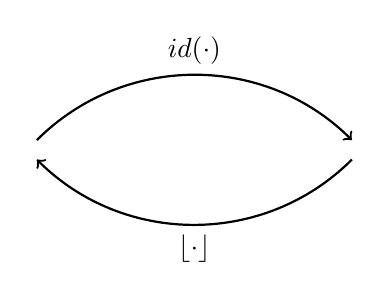
\begin{tikzpicture}
    \node (setA) at (-2,0) {$\Z$};
    \node (setB) at (2,0) {$\R$};

    \draw[->, thick] (setA.north) to[out=45, in=135] node[above] {$\text{id}(\cdot )$} (setB.north);

    \draw[<-, thick] (setA.south) to[out=-45, in=-135] node[below] {$\left\lfloor \cdot  \right\rfloor$} (setB.south);
\end{tikzpicture}
\end{center}

Żeby pokazać, że $(\id,\left\lfloor \cdot  \right\rfloor)$, trzeba pokazać, że 

\[
\begin{array}{c}
	 \id(n) \le x \\
	\hline\hline
	 n \le \left\lfloor x \right\rfloor 
\end{array}
.\] 

Podwójna linia oznacza obustronne wyprowadzenie(logiczna równoważnośći?).
\begin{proof}
	
	Implikacja w obie strony.

	Ustalmy dowolne $n \in \N$ oraz $x \in \R$. 
	
	$(\implies)$

	Załóżmy, że $\id(n) \le x$, czyli $n \le x$. Z własności funkcji podłoga, tzn $n \le x \implies n\le \left\lfloor x \right\rfloor) $, wynika, że $n \le \left\lfloor x \right\rfloor$
	
	$(\impliedby)$

	Załóżmy, że $n \le \left\lfloor x \right\rfloor$. Wtedy z definicji funkcji id, $\id(x) \le \left\lfloor x \right\rfloor$, następnie z własności funkcji podłoga $\id(x) \le x$
\end{proof}


Prosty przykład, w którym korzystamy z połączenia Galois. Pokażemy własność funkcji podłoga, tj $\left\lfloor x + n \right\rfloor = \left\lfloor x \right\rfloor + n$, gdzie $x \in \R, n \in \N$. Dzięki temu, że między $\R$ i $\N$ istnieje połączenie Galoisa, nie będziemy w ogóle korzystali z własności funkcji podłoga. 

\begin{lemma}
	Dla dowolnego $x \in \R$ zachodzi $\left\lfloor x \right\rfloor \le  x$
\end{lemma}
\begin{proof}
	Skorzystamy, z tego, że $(\id, \left\lfloor \cdot  \right\rfloor)$ tworzą połączenie Galois. Mianowicie
	\[
	\id (n) \le  y \iff n \le \left\lfloor y \right\rfloor
	.\] 

	Ustalmy dowolny $x \in \R$.

	Niech $n = \left\lfloor x \right\rfloor$ oraz $k = x$.

	Na mocy połączenia Galois, prawdziwa jest równoważność
	 \[
	\left\lfloor x \right\rfloor \le x \iff \left\lfloor x \right\rfloor \le \left\lfloor x \right\rfloor
	.\] 

	Ponieważ prawa strona równoważności jest spełniona trywialnie, 
	więc lewa też jest spełniona.
\end{proof}
\begin{proof}{$\left\lfloor x + n \right\rfloor = \left\lfloor x \right\rfloor + n$ dla każdego $x \in \R$ i $n \in \N$}
		\[
		\text{Połączenie Galoisa: } 
	\id (k) \le  y \iff k\le \left\lfloor y \right\rfloor
		.\] 	
		Ustalmy dowolny $x \in \R$ oraz $n \in \N$. 
		
		$\left( \le  \right)$ 
	
		Niech $k = \left\lfloor x \right\rfloor + n$ oraz $y = x + n$

		Na mocy Lematu 1. $\left\lfloor x \right\rfloor \le x$, zatem $\left\lfloor x \right\rfloor + n \le x + n$.

		Połączenia Galoisa mówi nam, że \[
		\left\lfloor x \right\rfloor + n \le   x + n \iff \left\lfloor x \right\rfloor + n \le \left\lfloor x+n \right\rfloor
		.\] 

		Ponieważ, lewa strona równoważności jest spełniona, więc zachodzi $\left\lfloor x \right\rfloor + n \le  \left\lfloor x+n \right\rfloor$

		($\ge$)
	
		Niech $k = \left\lfloor x+n \right\rfloor - n$ oraz
		$y = x$.

		Na mocy lematu 1.  $\left\lfloor x + n \right\rfloor \le x + n$, co jest równoważne temu, że $\left\lfloor x + n \right\rfloor - n \le  x$. 

		Połączenie Galoisa mówi nam, że 
		\[
		\left\lfloor x+n \right\rfloor-n \le x \iff \left\lfloor x+n \right\rfloor - n \le  \left\lfloor x \right\rfloor
		.\] 

		Ponieważ prawa strona równoważności jest spełniona, więc zachodzi $\left\lfloor x+n \right\rfloor - n \le  x$, czyli $\left\lfloor x + n \right\rfloor \le  \left\lfloor x \right\rfloor + n$
		

Ponieważ $\left\lfloor x + n \right\rfloor \le  \left\lfloor x \right\rfloor + n$
oraz 
$\left\lfloor x \right\rfloor + n \le  \left\lfloor x+n \right\rfloor$

wnioskujemy, że 
\[
\left\lfloor x \right\rfloor + n =  \left\lfloor x+n \right\rfloor
.\] 

\end{proof}

\begin{lemma}{Ko-ekstensywność operatora wnętrza}

	Mamy dwa posety: $\left( A, \le _A \right) $ oraz $\left( B, \le _B \right)$ i dwie funkcje: $f: A \rightarrow B$ oraz $g: B \rightarrow A$.

	Załóżmy, że $f$ i  $g$ tworzą połączenie Galois. 

	Wtedy dla dowolnych $x\in A$ oraz $y \in B$
	\[
	f(g(y)) \le_B  y
	.\] 
\end{lemma}
\begin{proof}
	
	Ustalmy dowolny $y \in B$. Niech $x = g(y)$. Funkcje $f$ i $g$ tworzą połączenie Galoisa:
	\[
	f(x) \le _B y \iff x \le_A g(y)
	.\]

	$x = g(y)$, zatem z zwrotności relacji $\le _A$ wnioskujemy, że prawa strona równoważności jest zawsze prawdziwa. Zatem lewa strona jest zawsze prawdziwa, czyli 
	\[
	f(g(y)) \le _B y
	.\] 
\end{proof}
\begin{lemma}{Ekstensywność operatora domknięcia}
	
	Mamy dwa posety: $\left( A, \le _A \right) $ oraz $\left( B, \le _B \right)$ i dwie funkcje: $f: A \rightarrow B$ oraz $g: B \rightarrow A$.
	Załóżmy, że $f$ i  $g$ tworzą połączenie Galois 

	Wtedy dla dowolnych $x\in A$ oraz $y \in B$
	\[
		x \le _A g (f (x))
	.\] 
\end{lemma}
\begin{remark}

	To, że funkcje tworzące połączenie Galoisa są homomorfizmami nie jest dodatkowym założeniem, a nieuniknioną konsekwencją powyższej definicji. 
\end{remark}

\begin{proof}{Jeśli dwie funkcje określone na posetach tworzą połączenie Galois, to są one homomorfizmami}
	
	Niech $\left( A, \le _A \right) $ i $\left( )B, \le _B \right) $ będą posetami oraz $f: A \rightarrow B$ i $g: B \rightarrow A$ funkcjami tworzącymi połączenie Galois.

	\textbf{Dowód dla funkcji f} 

	Ustalmy dowolne $a_1,a_2 \in A$. Pokażemy, że zachodzi warunek
	\[
	a_1 \le _A a_2 \implies f(a_1) \le _B f(a_2)
	.\] 
	
	Załóżmy, że $a_1\le _A a_2$.

	Z lematu 3. mamy $a_2 \le A g(f(a_2))$. Z założenia, mamy $a_1 \le_A a_2$. Zatem z przechodniości relacji $\le _A$ wnioskujemy, że $a_1 \le _A g(f(a_2)$. 

Korzystając z połączenia Galois, powyższy warunek jest równoważny $f(a_1) \le _A f(a_2)$

\textbf{Dowód dla funkcji g}

	Ustalmy dowolne $b_1,b_2 \in B$. Pokażemy, że zachodzi warunek
	\[
	b_1\le _B b_2 \implies g(b_1) \le _A g(b_2)
	.\] 

	Załóżmy, że $b_1\le _B b_2$. 

	Z lematu 2, mamy $f(g(b_1)) \le _B b_1$. Korzystając z założenia oraz przechodniości relacji $\le _B$, wnioskujemy, że $f(g(b_1)) \le _A b_2$. Następnie z tego, że f i g tworzą połączenie Galois, tj
	\[
	f(g(b_1)) \le_B b_2 \iff g(b_1) \le_A g(b_2)
	.\] 

	Wnioskujemy, że $g(b_1) \le _A g(b_2)$.
\end{proof}
Co możemy powiedzieć o wyniku, jeśli podwójnie nałożymy złożenie gf?

Dwukrotne nałożenie złożenia gf nic nie zmienia w stosunku do jednokrotnego nałożenia.
\begin{lemma}
	Niech $(A, \le _A)$ i $(B, \le _B)$ będą posetami oraz $f: A \rightarrow B$ i $g: B \rightarrow A$ będą funkcjami, które tworzą połączenie Galoisa. Wtedy
	\[
	g(f(g(f x))) \le  g (f x)
	.\] 
\end{lemma}
\begin{proof}

	Lemat 2. mówi nam, że dla dowolnego $y\in B$ jest $f(g(y)) <_B y$

	Zatem z lematu 2. otrzymujemy
	\[
	f(g(b)) \le _B b \text{, czyli } f(g(f(x))) \le _B f(x)
	.\] 

Ponieważ funkcja $g$ jest homomorfizmem więc zachowuje porządek, zatem \[
g(f(g(f(x)))) \le _B g(f (x))
.\] 
\end{proof}

Inny przykład:

Niech $A,B $ będą dowolnymi zbiorami oraz $f:A \rightarrow B $ dowolną funkcją.

Mamy:

\begin{center}
$
 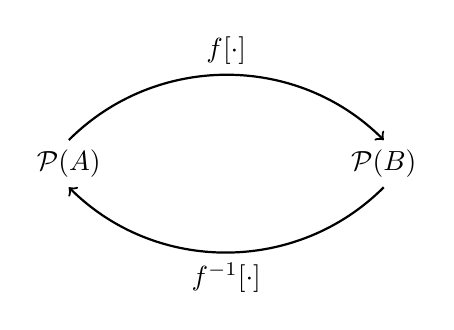
\begin{tikzpicture}
	 \node (setA) at (-2,0) {$\mathcal{P}(A)$};
	 \node (setB) at (2,0) {$\mathcal{P}(B)$};
 
	 \draw[->, thick] (setA.north) to[out=45, in=135] node[above] {$f[\cdot ]$} (setB.north);
 
	 \draw[<-, thick] (setA.south) to[out=-45, in=-135] node[below] {$f^{-1}[\cdot ]$} (setB.south);
 \end{tikzpicture}$
\end{center}

gdzie: $f[X]$ to obraz zbioru $X \subseteq \mathcal{P}(A)$ przez funkcję f, a  $f^{-1}[Y]$ to przeciwobraz zbioru $Y\subseteq \mathcal{P}(B)$ przez funkcję f.

Pokażemy, że $f[\cdot ]$ oraz $f^{-1}[\cdot ]$ tworzą połączenie Galois, czyli 
\[
	 f[X] \subseteq Y \iff X \subseteq f^{-1}[Y]
.\] 
\begin{proof}

	Pokażemy implikacje w obie strony. Niech $X \subseteq \mathcal{P}(A)$ oraz $Y \subseteq \mathcal{P}(B) $.

	$\left( \implies \right)$ 

	Załóżmy, że $f[X] \subseteq  Y$. Chcemy pokazać, że $X \subseteq f^{-1}[Y]$

	Ustalmy dowolny $x\in X$. Wtedy $y = f(x) \in f[X]$, korzystając z założenia wnioskujemy, że $y \in Y$. Zatem $x \in f^{-1}[Y]$ 
	a co za tym idzie $X \subseteq f^{-1}[Y]$.

	$\left( \impliedby \right) $ 
	
	Załóżmy, że $X \subseteq f^{-1}[Y]$. Chcemy pokazać, że $f[X] \subseteq  Y$.

	Ustalmy dowolny $y \in f[X]$. Wtedy istnieje takie $x_0 \in X$, że $f(x_0) = y$. Korzystając z założenia, otrzymujemy $x_0 \in f^{-1}[Y]$, a co za tym idzie $y = f(x_0) \in Y$. Zatem $f[X]\subseteq Y$ 

\end{proof}

\begin{definition}{Ekstensywność}
	
	Niech $(A, \le)$ będzie posetem oraz $f: \underline{A} \rightarrow \underline{A}$.

	Operator(funkcja) f jest \textbf{ekstensywny}, jeśli spełnia poniższy warunek:
	\[
	\left( \forall a \in A \right) a\le f(a)
	.\] 
\end{definition}

\begin{definition}{Idempotentność}
	
	Niech $(A, \le)$ będzie posetem oraz $f: \underline{A} \rightarrow \underline{A}$.
Operator(funkcja) f jest \textbf{idempotentny} jeśli spełnia poniższy warunek:
	\[
	\left( \forall a \in A \right)f(f(a)) \le  f(a) 	
	.\] 
\end{definition}

\begin{definition}{Operator domknięcia.}

	$\cl:\underline{X} \rightarrow \underline{X} $ jest operatorem domknięcia jeśli:
	\begin{itemize}
		\item jest homomorfizmem,
		\item jest ekstensywny,
		\item jest idempotentny.
	\end{itemize}
\end{definition}

\begin{theorem}
	
	Dowolny operator domknięcia $\cl:\underline{X} \rightarrow\underline{X} $ jest złożeniem pewnego połączenia Galois $(f,g)$ jako $\cl=g\circ f$.
\end{theorem}
\begin{proof}
	$\textbf(TODO)$
\end{proof}

\begin{definition}{Kresy górne i kresy dolne}

	TODO
\end{definition}

\begin{definition}{Ograniczenie górne.}
	
	TODO	
\end{definition}

\begin{definition}{Krata}
	
	Porządek $(P, \le )$ nazywamy kratą jeśli posiada element najmniejszy i element największy oraz gdy każdy skończony podzbiór zbioru $P$ zawiera kres górny oraz kres dolny.
\end{definition}

\begin{definition}{Krata zupełna}
	
	Porządek $\left( P, \le  \right) $ jest kratą zupełną, jeśli każdy podzbiór zbioru $P$ ma kres górny i kres dolny. ma kres górny i kres dolny.
\end{definition}
